\documentclass[10pt]{article}

\usepackage{parskip}
\usepackage[margin=1in]{geometry} 
\usepackage{amsmath,amsthm,amssymb, graphicx, multicol, array}
\usepackage{makecell}
\usepackage{enumitem}
\usepackage{amssymb}
\usepackage{float}
\usepackage{href-ul}
 
\newcommand{\N}{\mathbb{N}}
\newcommand{\Z}{\mathbb{Z}}
 
\newenvironment{problem}[2][Problem]{\begin{trivlist}
\item[\hskip \labelsep {\bfseries #1}\hskip \labelsep {\bfseries #2.}]}{\end{trivlist}}

\begin{document}
 
\title{Midterm}
\author{Jakob Sverre Alexandersen\\
GRA6551 Quantitative Risk And Asset Management}
\maketitle

% \tableofcontents
% \newpage
\section{Rolling zero-mean correlations of returns}
For the full sample, compute yearly rolling zero-mean correlations of returns between the energy and high-tech sector. This is done as follows: at each date $t $ (excluding the first 252 days), compute the correlation between the daily returns of the energy and high-tech sector, but using a zero-mean rather than the sample mean. This correlation is then: 
\begin{gather*}
    \rho_t = \frac{\frac{1}{252}\sum_{j = 1}^{252}R_{E, t - j}R_{HT, t - j}}{\sqrt{\frac{1}{252}\sum_{j = 1}^{252}R^2_{E, t - j}}\sqrt{\frac{1}{252}\sum_{j = 1}^{252}R^2_{HT, t - j}}}
\end{gather*}

\begin{enumerate}
    \item Rolling correlation plot
    \begin{figure}[H]
        \centering
        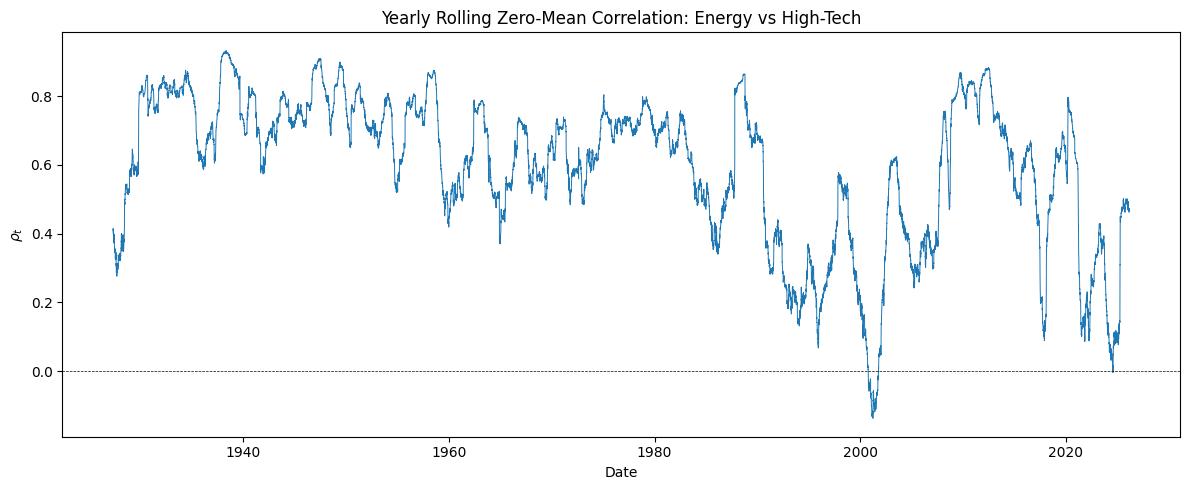
\includegraphics[width=1\textwidth]{2026-04-10-15-22-16.png}
    \end{figure}
    \item Compute its mean, median, q 0.05 and q 0.95

    This was done using simple \verb|np| functions: 

    \begin{center}
        \begin{tabular}{|c|c|c|c|}
            \hline 
            \textbf{mean} & \textbf{median} & \textbf{q 0.05} & \textbf{q 0.95}\\\hline 
            0.601 & 0.656 & 0.182 & 0.861 \\\hline
        \end{tabular}
    \end{center}
    \newpage
    \item Repeat 1-2 with a 5-year rolling correlation
    \begin{figure}[H]
        \centering
        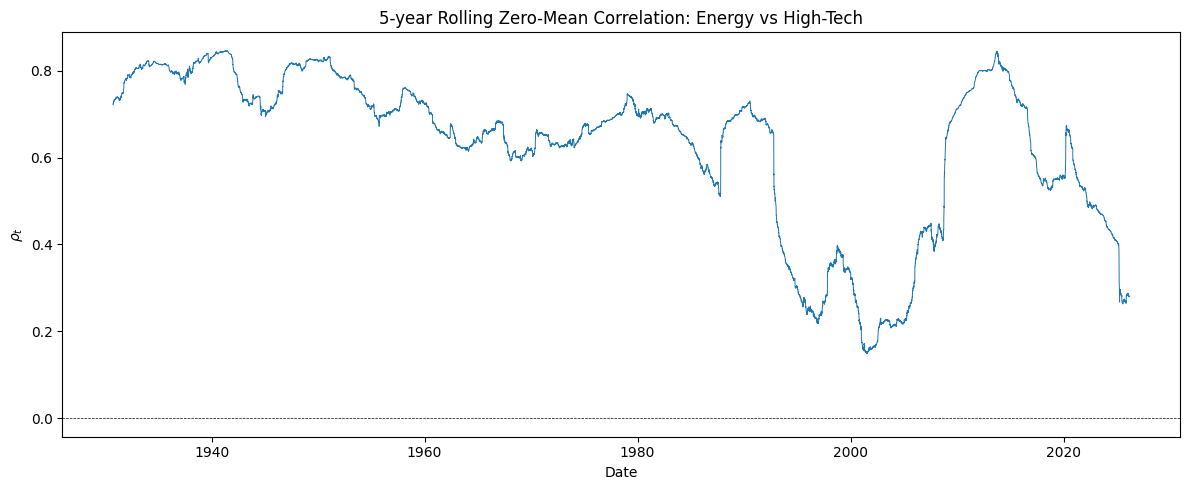
\includegraphics[width=1\textwidth]{2026-04-10-15-43-50.png}
    \end{figure}
    \begin{center}
        \begin{tabular}{|c|c|c|c|}
            \hline 
            \textbf{mean} & \textbf{median} & \textbf{q 0.05} & \textbf{q 0.95}\\\hline 
            0.634 & 0.685 & 0.236 & 0.824 \\\hline
        \end{tabular}
    \end{center}
    \item Briefly comment on the results

    
\end{enumerate}
\end{document}